\chapter{Implementation}\label{implementation}\label{implem_ch}
This Chapter describes the implementation process of the design from the previous chapter. All non trivial issues will be described for both the wristband and companion app. The end of the Chapter will shorty describe the testing process that was done during the implementation.

\section{Proof of Concept}
Before the actual implementation of the design from the previous Chapter, a Proof of Concept (PoC) was created. This had several purposed, most importantly to see if it was at all possible to have at least some sense of the scale when performing the gestures. The component listed bellow was connected together as shown in Figure \ref{sketch_bb} and \ref{sketch_schem}, the finished PoC can be seen in Figure \ref{poc}.

\begin{itemize}
    \item Adafruit Feather M0 Adalogger\cite{adalogger} with a 350mAh 3.7V battery
    \item Adafruit 9-DOF Absolute Orientation IMU Fusion Breakout - BNO055\cite{gyro}
	\item Flora Wearable Bluefruit LE Module\cite{bluefruit}
	\item A push button
	\item A 100k$\Omega$ resistor
\end{itemize}

The Feather M0 Adalogger was controlled by an Arduino script, that after establishing a bluetooth connection waits for the button to be pressed. When the button is pressed the Euler angles from the IMU is read, and transmitted over the bluetooth connection, the LED is connected to the switch so it will light up as long as the button is pressed. A simple GUI (as seen in Figure \ref{poc_s1}) was created using a Python script, that connected to the bluetooth module and when receiving data displayed the raw values and the mapped scaled value between zero and ten using the mapping function seen in Equation \ref{eq_roll} (the scaled value was rounded for simplicity). Only the wrist gesture was tested using the PoC, if the PoC proved the wrist gesture to be possible the arm gesture would too, since the wrist gesture is much finer than the arm gesture. Both the Arduino and Python scrips are linked to in Appendix \ref{poc_code}.

\begin{figure}[h!]
    \centering
    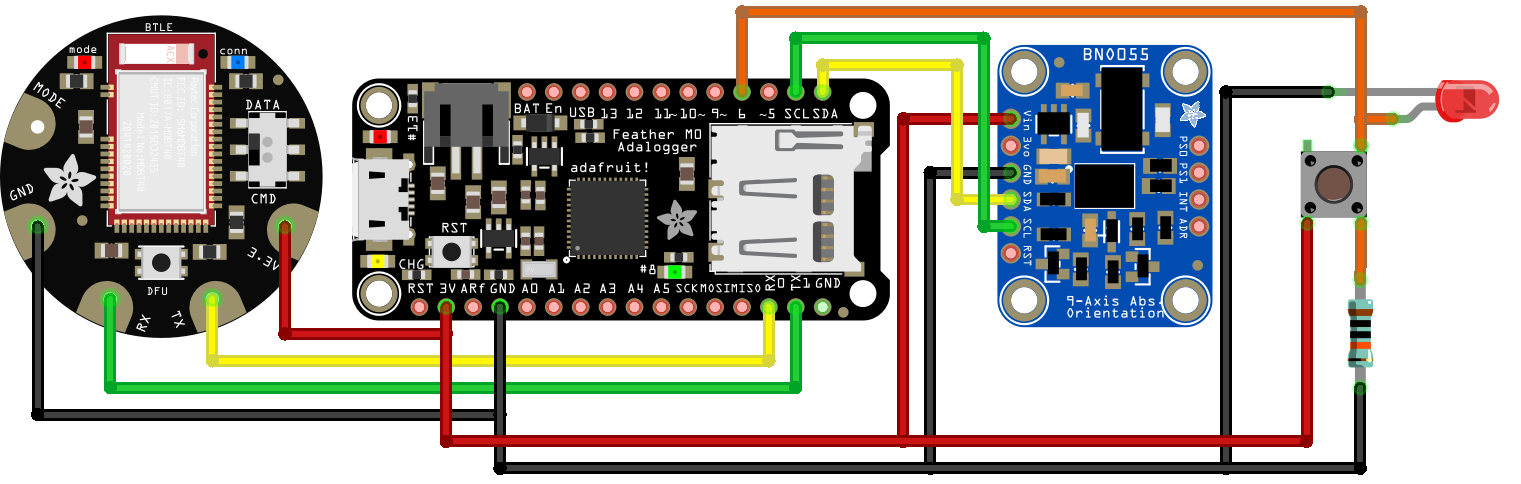
\includegraphics[width=1\textwidth]{figures/Sketch_bb.png}
    \caption{Wiring for of the proof of concept. Battery not shown}
    \label{sketch_bb}
\end{figure}

\begin{figure}[h!]
    \centering
    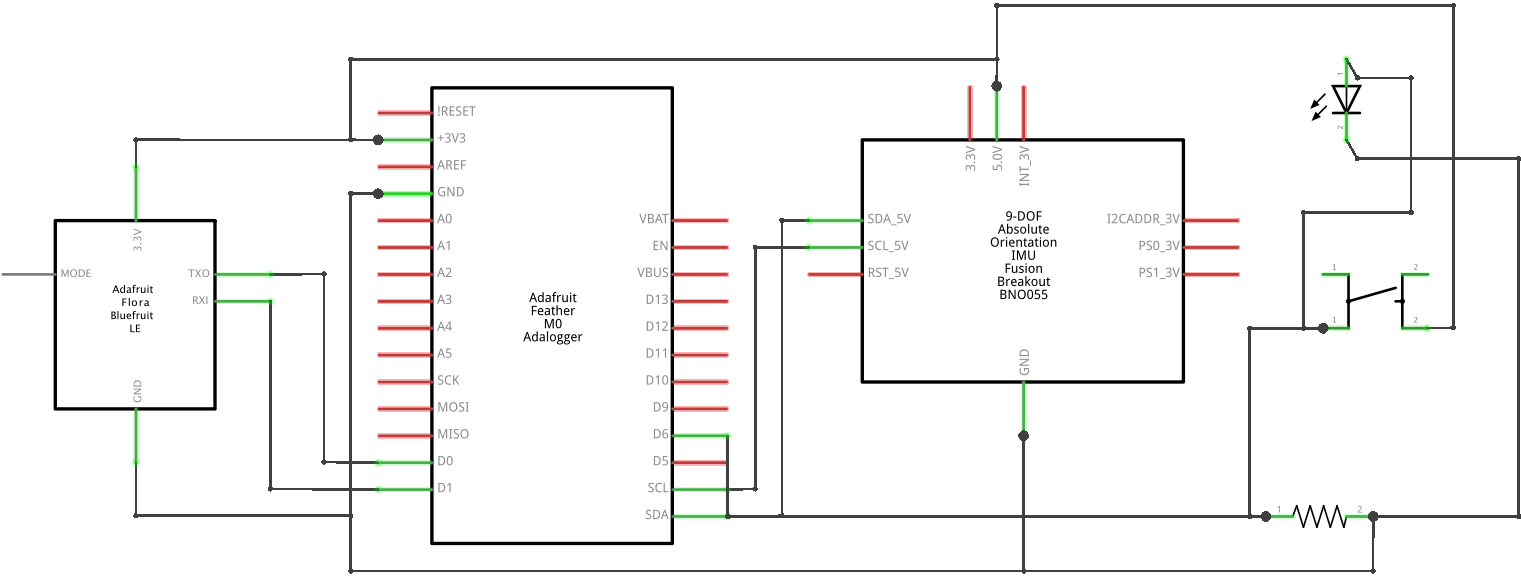
\includegraphics[width=1\textwidth]{figures/Sketch_schem.png}
    \caption{Schematic for the proof of concept. Battery not shown}
    \label{sketch_schem}
\end{figure}

\begin{figure}[h!]
    \centering
    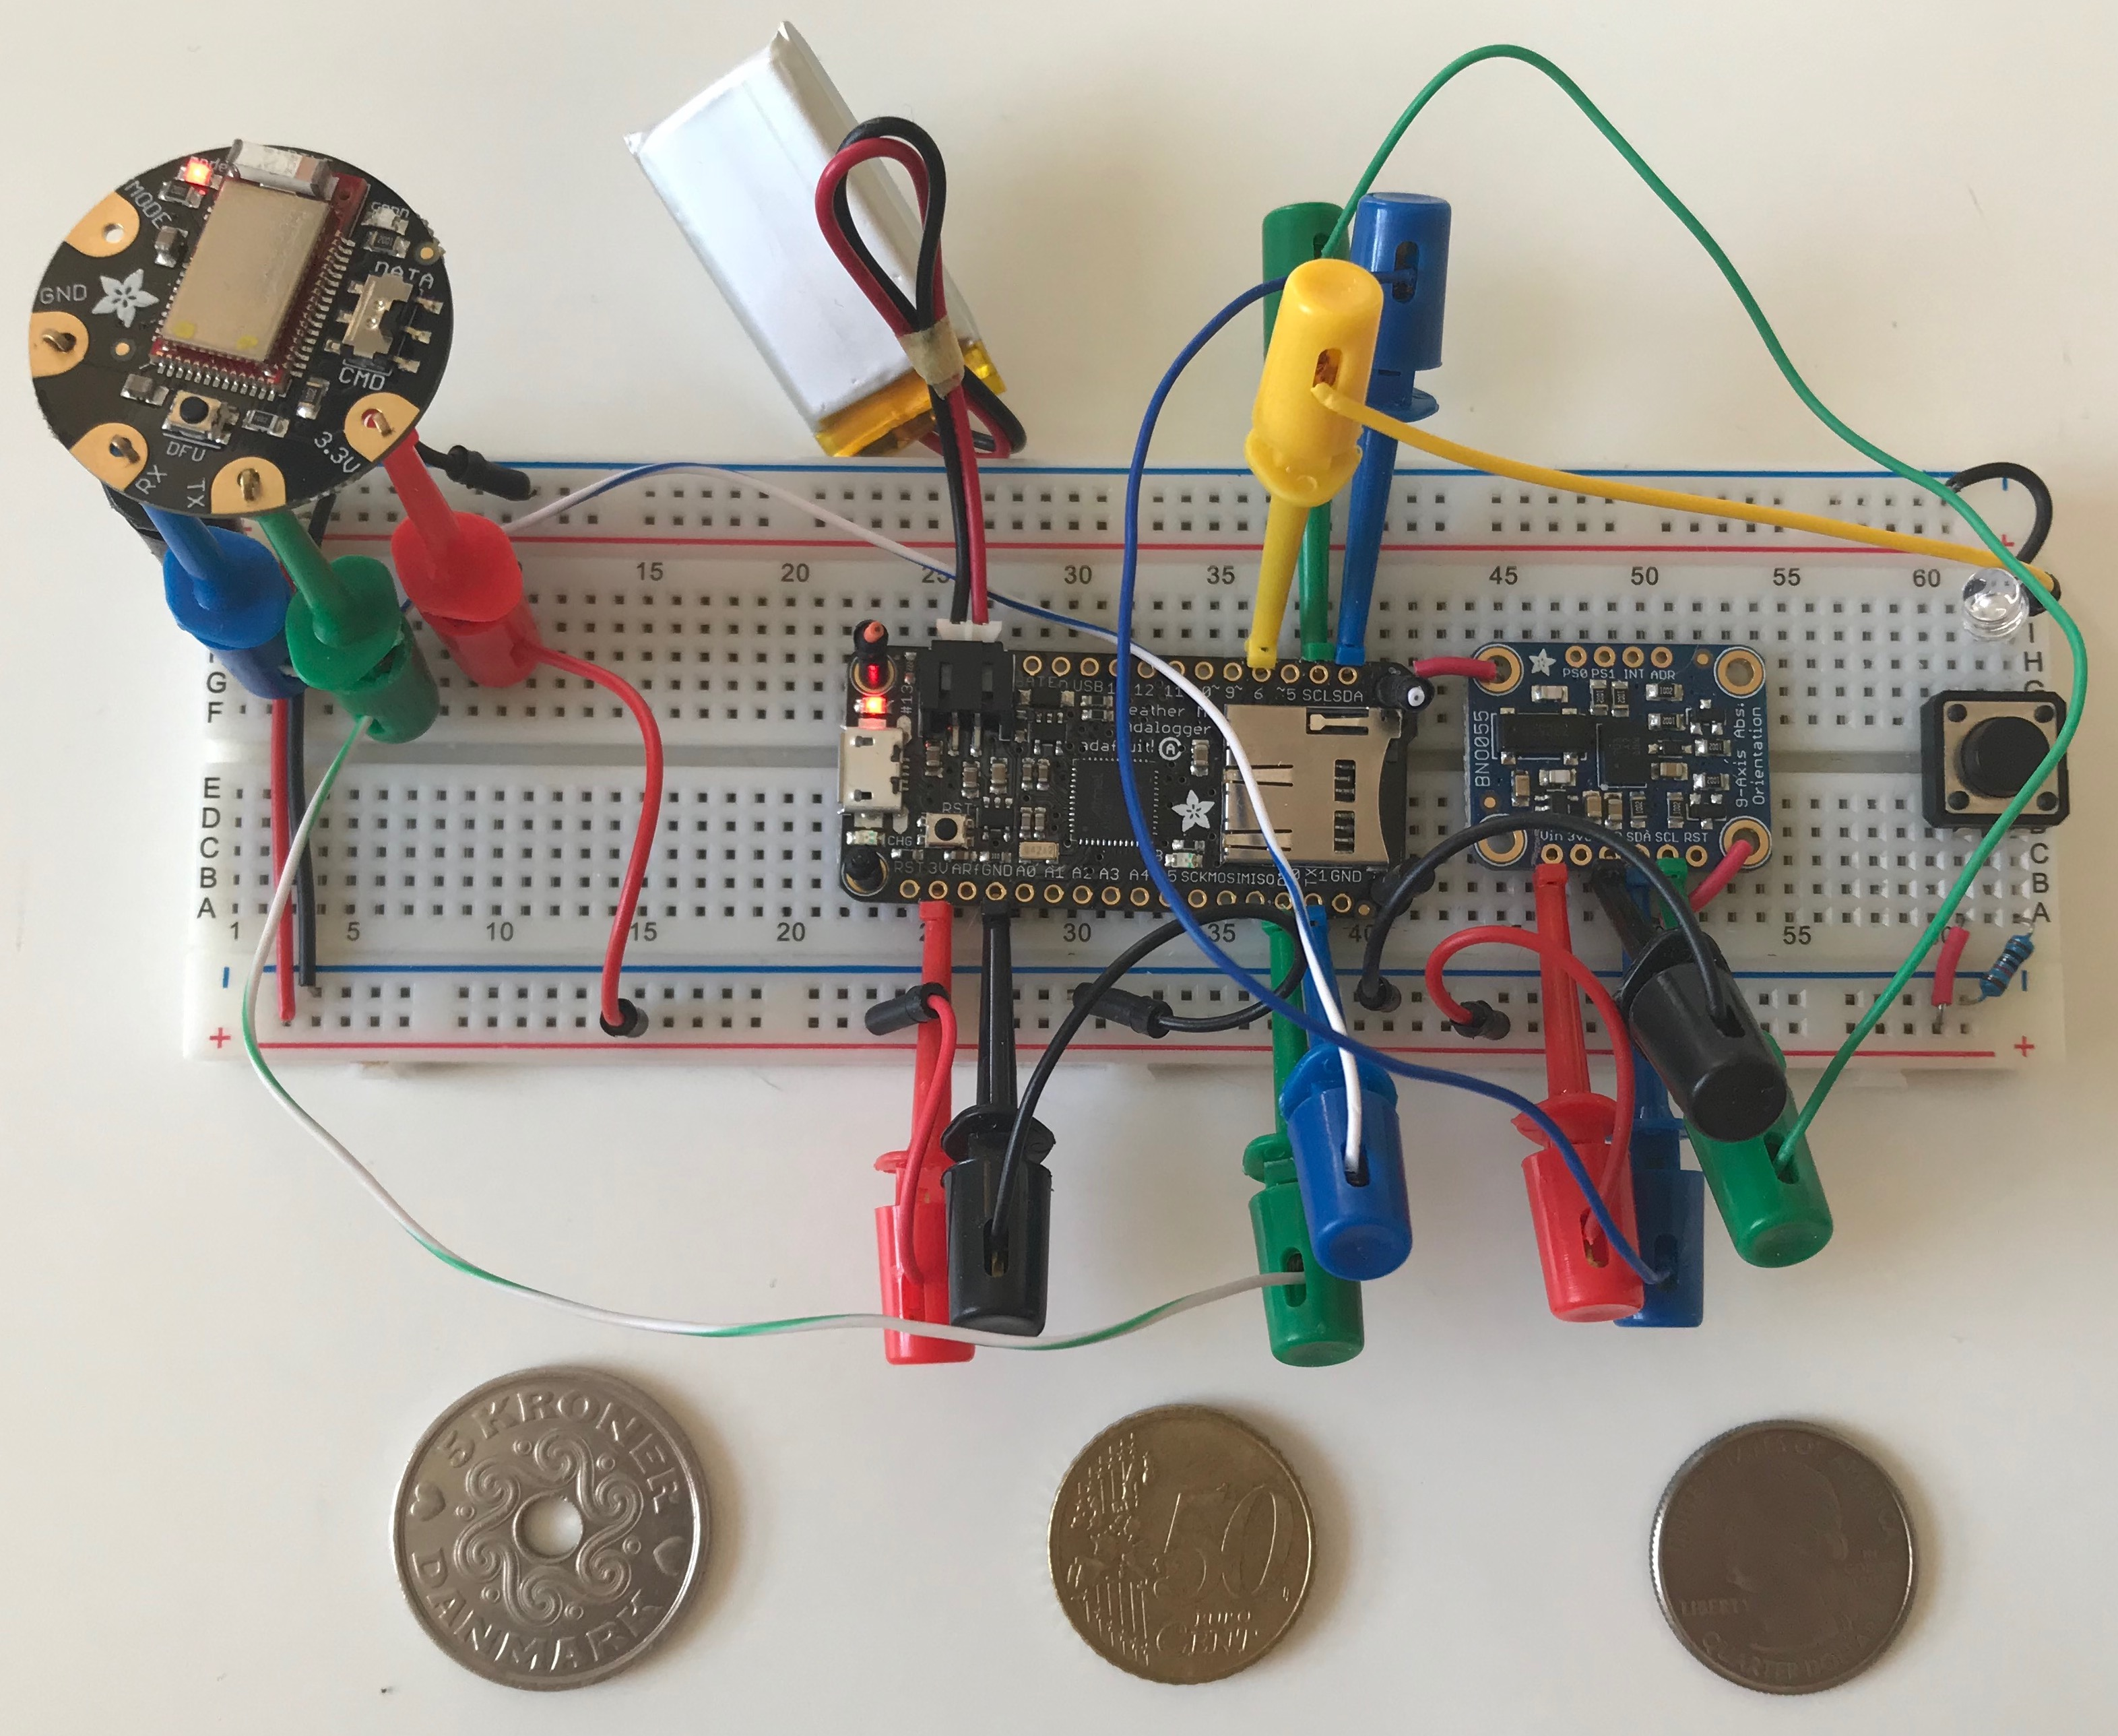
\includegraphics[width=0.6\textwidth]{figures/poc.jpg}
    \caption{Proof of concept. Components from left to right on the breadboard: Bluefruit LE Module, Feather M0 Adalogger and battery, IMU Fusion Breakout - BNO055, push button and led. Coins below for scale (5dkk, 0.5\EURtm{} \& 0.25\$)}
    \label{poc}
\end{figure}

The first thing that was tested using the PoC was sensor drift, since it was important to prevent this. A test was preformed logging the Euler angles with and without calibration while the IMU sat completely still. Once every minute the Euler angles was read from the IMU and logged to a file. Two trials where run, one for nine hours and one for twelve hours without and with calibration respectively. The results can be seen in Figure \ref{drift1} and \ref{drift2}, we see that without calibration the sensor drifts and the Euler angles change quite dramatically over time, while with calibration the Euler angles only had minor change. This concluded that with proper calibration sensor drift would not be an issue.

\begin{figure}[h!]
    \centering
    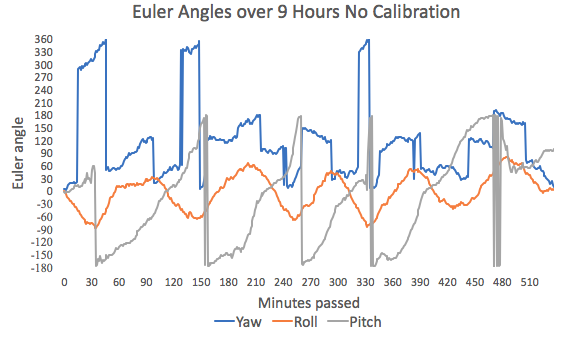
\includegraphics[width=1\textwidth]{figures/drift1.png}
    \caption{Reading the Euler angles from the BNO055 IMU\cite{gyro} without calibration}
    \label{drift1}
\end{figure}

\begin{figure}[h!]
    \centering
    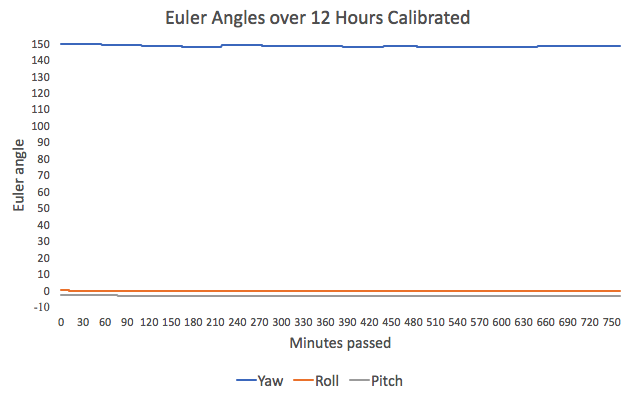
\includegraphics[width=1\textwidth]{figures/drift2.png}
    \caption{Reading the Euler angles from the BNO055 IMU\cite{gyro} with calibration}
    \label{drift2}
\end{figure}



The PoC was then tested by strapping it to the back of the lower arm using rubber bands, then moving the arm to different positions using the wrist gesture and pressing the button. It was validated that the concept worked, and it was possible to input different values using the gesture. The question still remained how precise it was. At this point the author thought that this concept would only be precise enough to be used on a three point scale and would not be able to compete with a VAS.

\begin{figure}[h!]
    \centering
    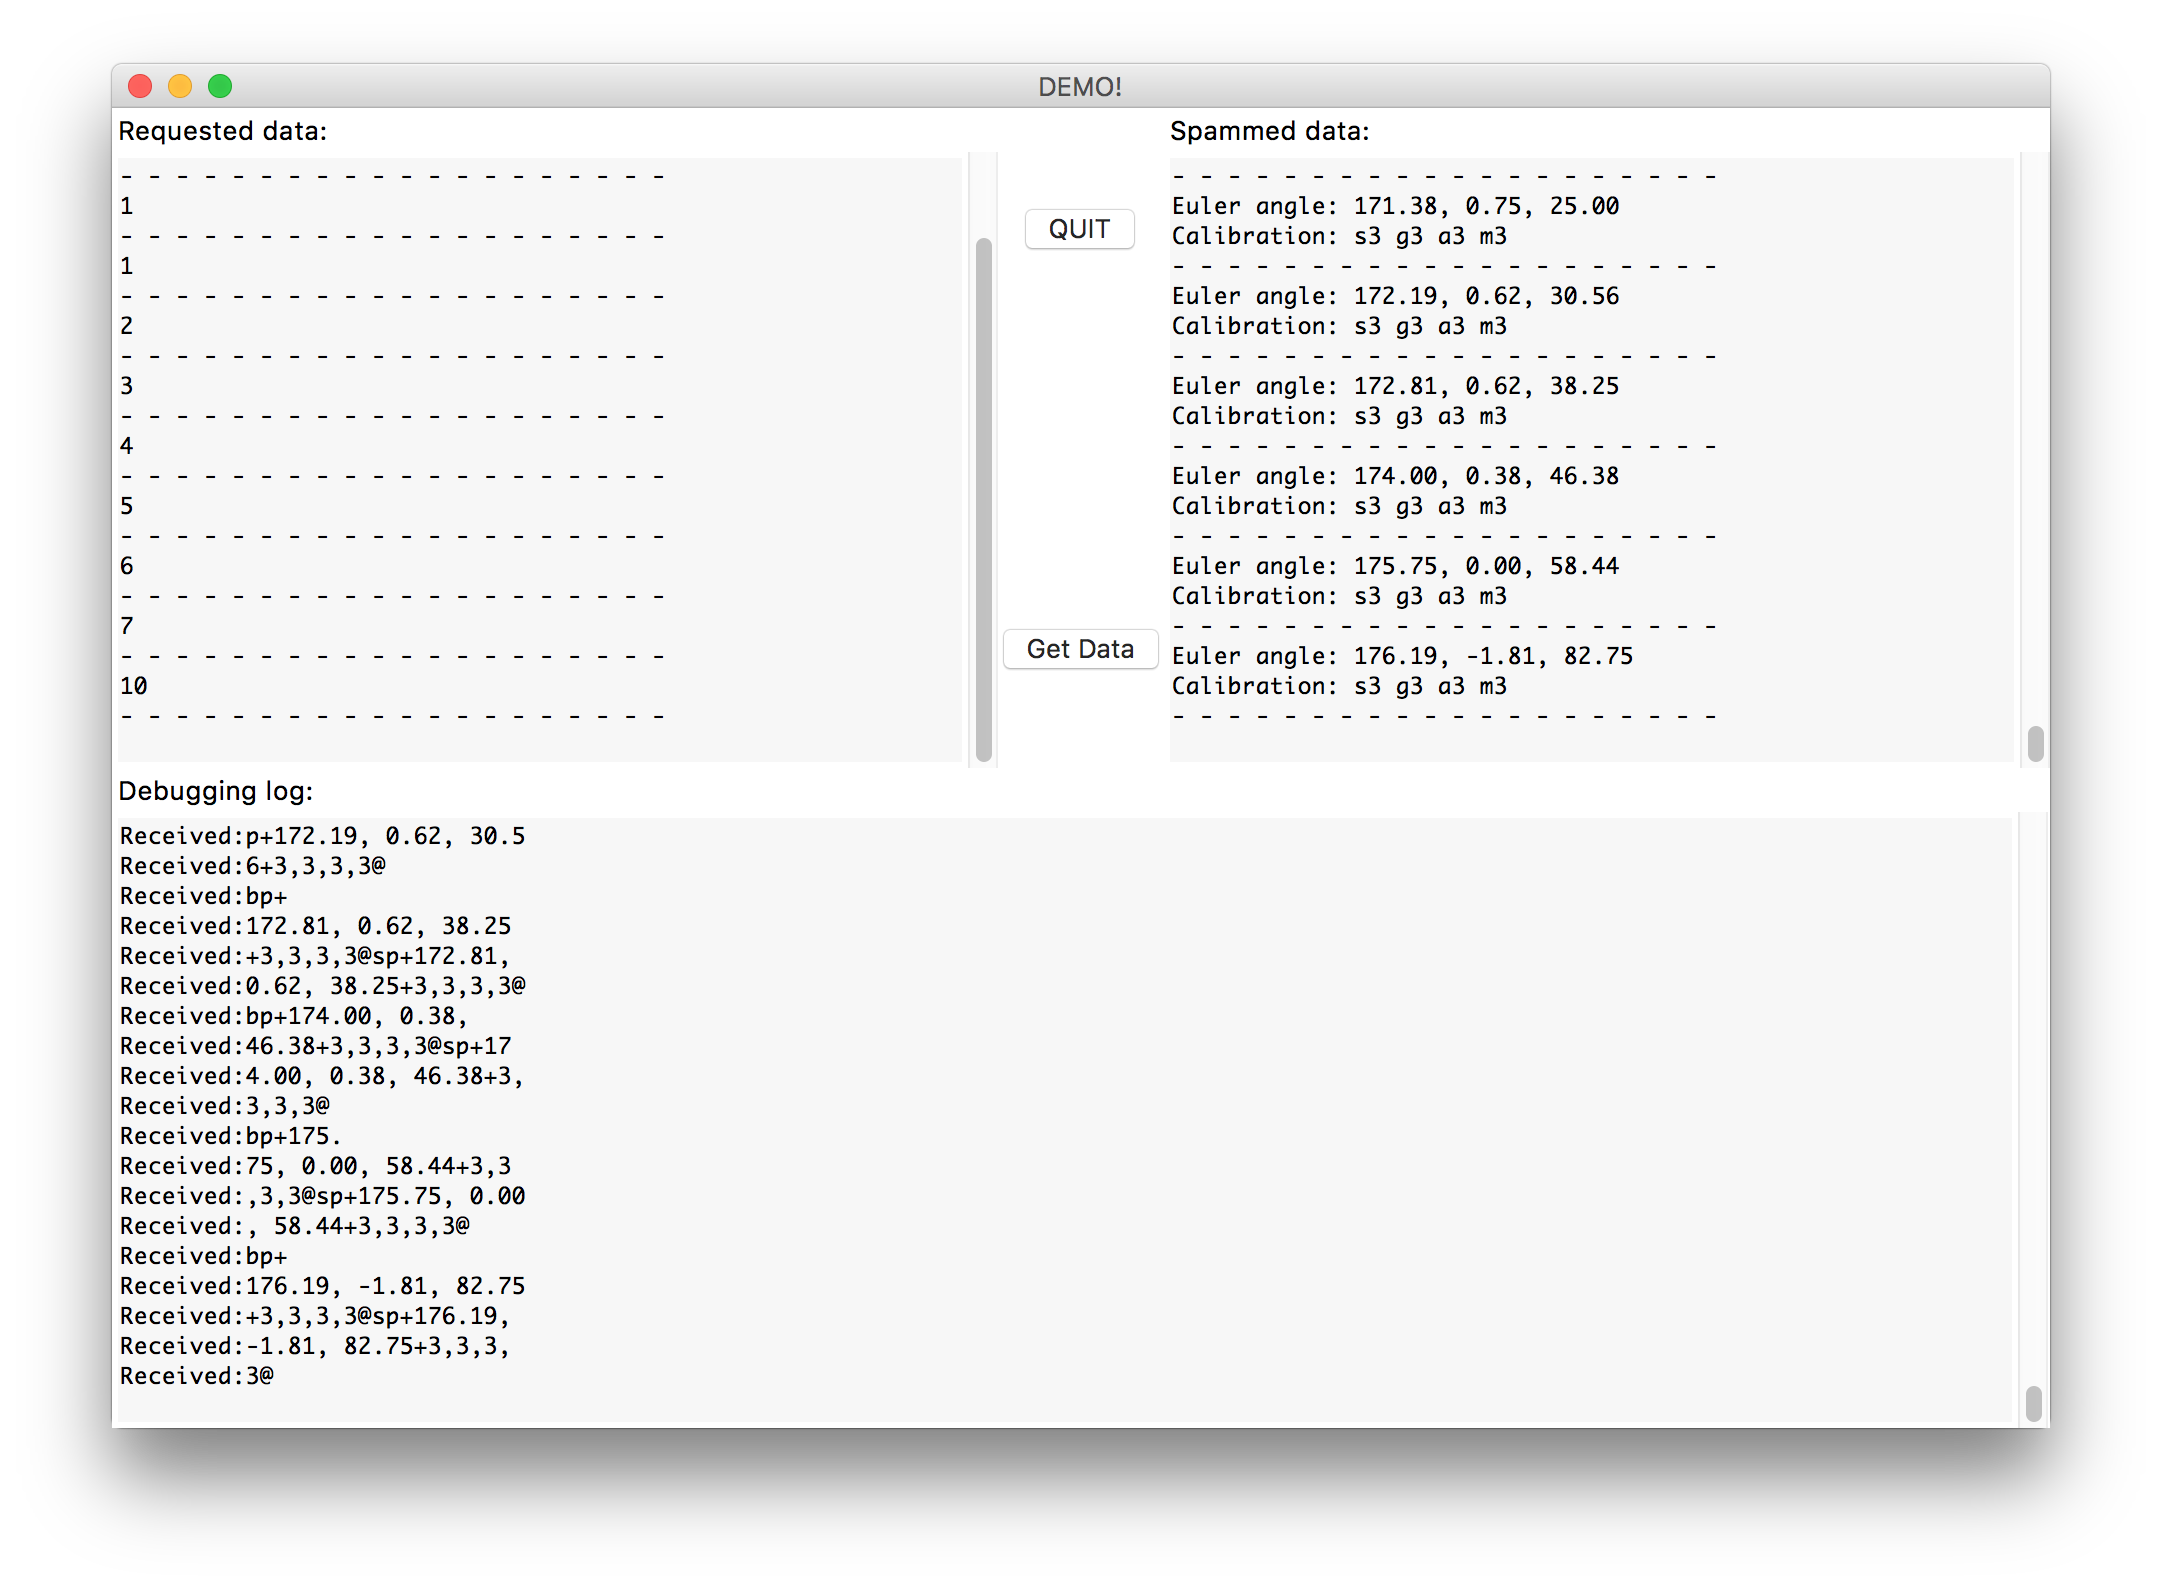
\includegraphics[width=1.2\textwidth]{figures/poc_s1.png}
    \caption{PoC GUI. Top left shows the data mapped to the 0-10 scale. Top right shows the raw data and calibration. Bottom shows a debug log}
    \label{poc_s1}
\end{figure}


\section{Prototype}
With the PoC being a success the design from Chapter \ref{design_ch} could be implemented. The components used for the PoC could in theory be rearranged and soldered together into a more compact design, but in practice it would be quite bulky for a wristband device. Instead a small device called \say{MetaMotionR} created by mbientlab\cite{mbient} was used. The device is roughly the same size as a regular wrist watch, although thicker, and is packed with sensors, most importantly an IMU with the same Sensor Fusion algorithm as the BNO055. The MetaMotionR is also equipped with a push button and has Low Energy Bluetooth built in, making it an excellent hardware choice for this implementation.

\begin{figure}[h!]
    \centering
    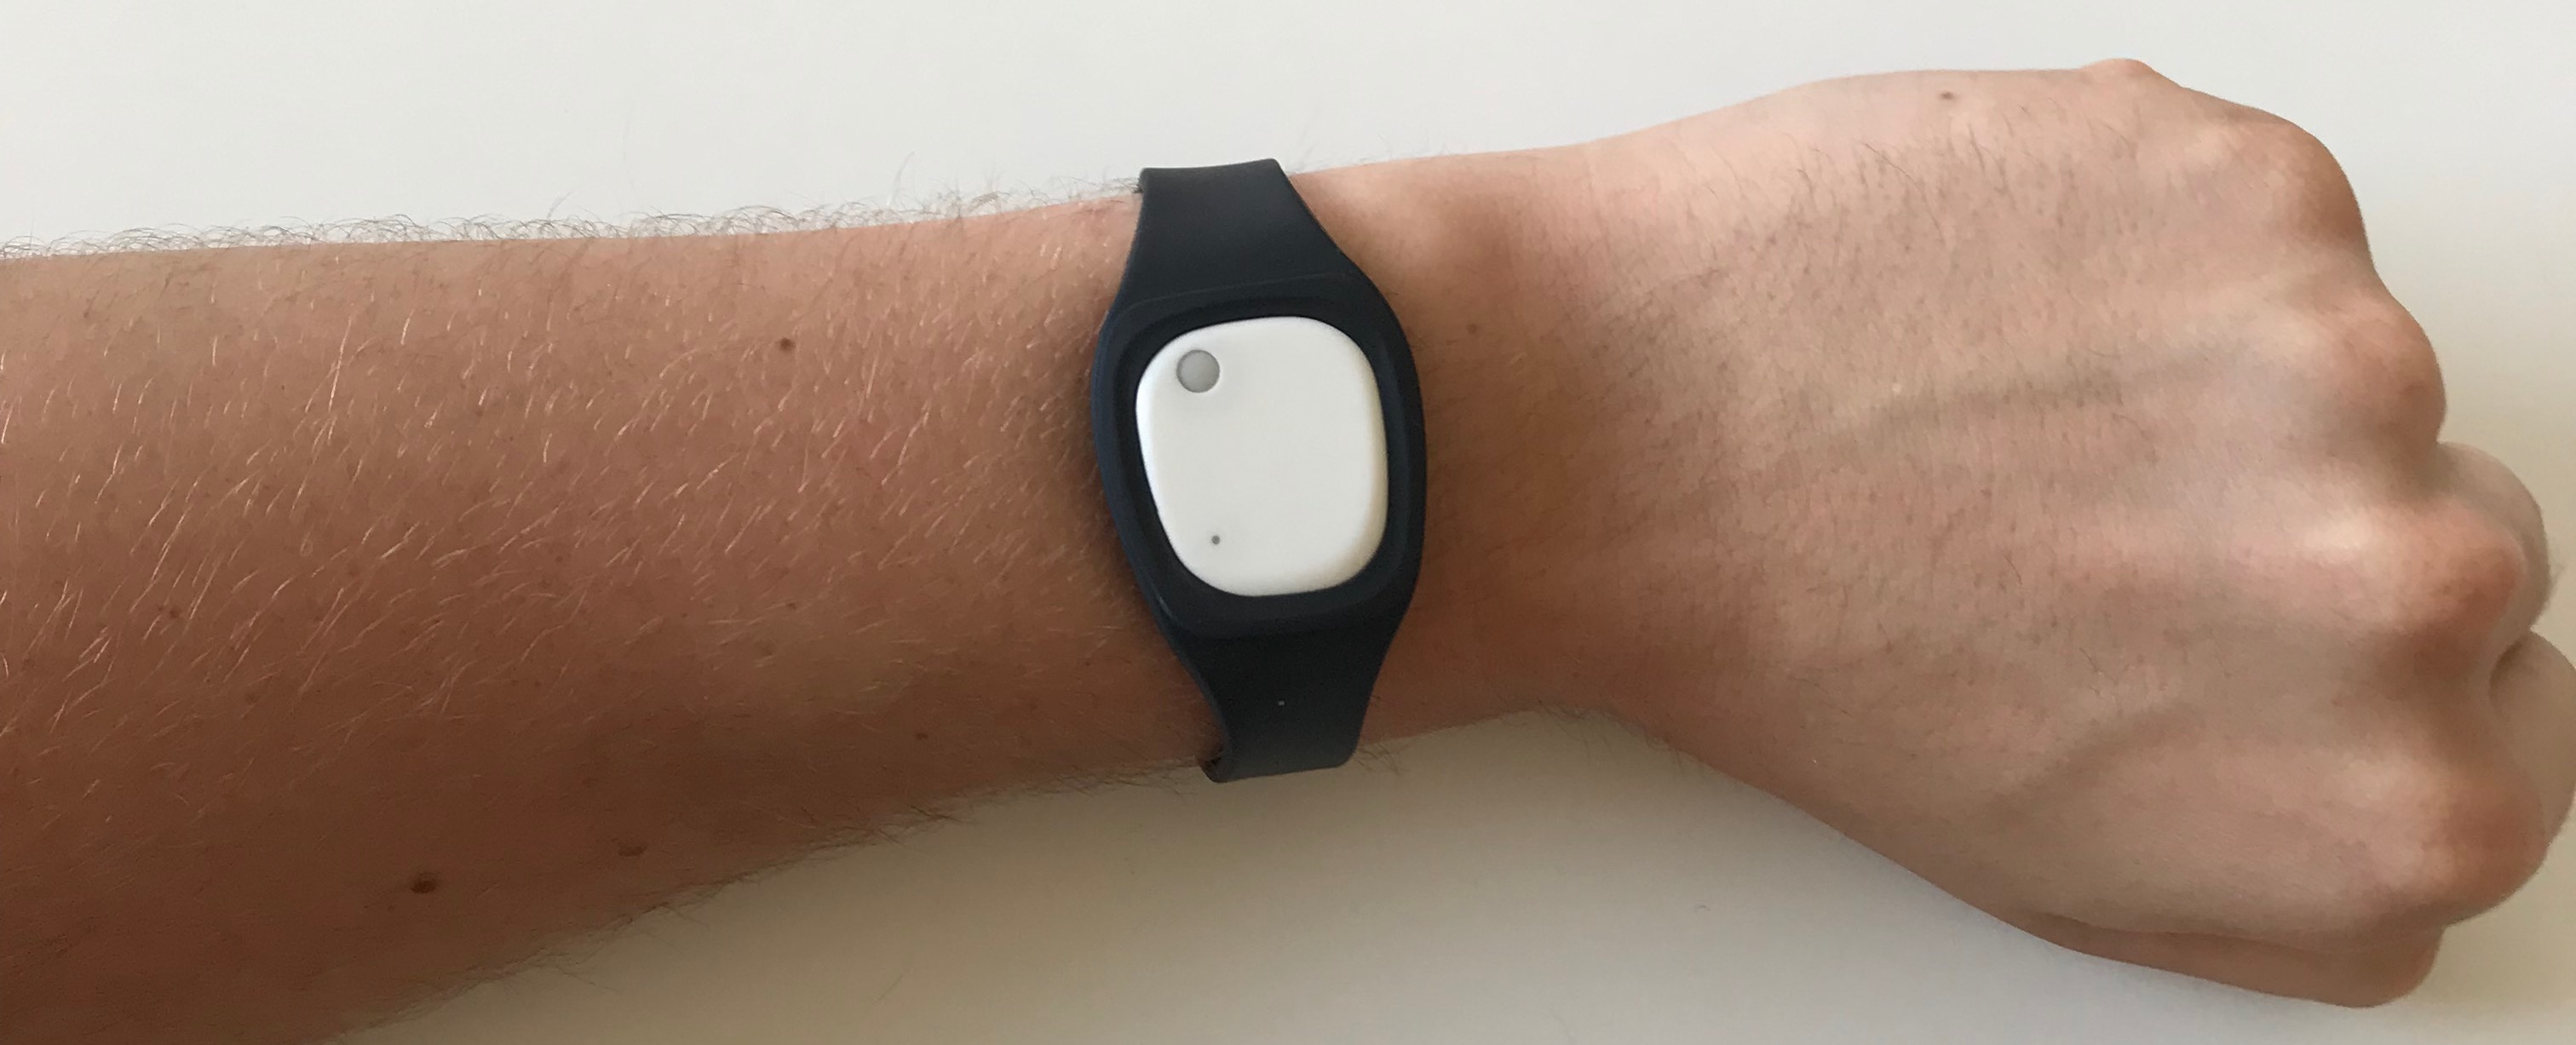
\includegraphics[width=0.6\textwidth]{figures/mbient.jpg}
    \caption{MetaMotionR by mbientlab\cite{mbient}}
    \label{mbient}
\end{figure}

The MetaMotionR must be programmed using mbientlab's API, available for several platforms\cite{api_mbient}. Since the design all ready requires a companion app for the wristband the API for Android will be used. The MetaMotionR has 8MB of flash memory which can be used to store commands and log data, it allows for more than 200.000 log entries when logging Euler angles, which should be more than enough for this use case. The MetaMotionR is programmed to run the Sensor Fusion algorithm and whenever the button us pressed it will log the current orientation, turn its LED on and vibrate to give user feedback. It was considered to use the vibration motor to give varied feedback dependent on the value logged, but the vibration motor doesn't offer much customization, only the time interval can be customized, and if the vibration is any shorter than half a second it might not vibrate, therefore this idea was discarded for this implementation.

When the companion app connects to the MetaMotionR the logged data can be imported over the app and is afterwards deleted from the MetaMotionR to free up space for future data entries. Beside storing the Euler angles each data entry has a time stamp. The time on the MetaMotionR is synchronized whenever it connects to a smartphone. The Euler angles are measured with three decimals precision, which is much finer than the precision that can be achieved by using the gestures. One flaw with the MetaMotionR is that logged entries and the commands are stored in the flash memory, which requires power, this means that if the MetaMotionR runs of power all logged entries will be lost, and it needs to connect to the companion app before it can be used to log entries again. The battery life of the MetaMotionR will be explored later in this Chapter. 

\section{Companion App}
Following the requirements from Section \ref{requirements} the companion was implemented. The app was build upon mbientlab's Android tutorial \say{starter app}\cite{starter_mbient}. The starter app handles the bluetooth connectivity (searching for devices and connected), beside this the rest was left to be implemented. As explained the app programs the MetaMotionR, this happens every time the device connects to the app. The MetaMotionR is programmed to turn on its LED, log the Euler angles (saved to on board memory), vibrate the motor and turn the LED off again every time the button is pressed. Once programmed the MetaMotionR can run independently.

The app itself consist of three buttons, one to import, share and delete data. The largest part of the screen is reserved for displaying the data in a scroolable list, with the latest entry on top. When the data is imported from the device the Euler angles get mapped to the scaled value, this value together with the Euler angles, time stamps and battery percentage of the MetaMotionR are saved to internal file (in CSV format). The scaled values are displayed in the app together with its time stamp and battery percentage. The scaled value is color coded from green (low values) to yellow (middle values) to red (high values) as seen in Figure \ref{proto_s1}. The color coding was implemented using HTML formatting and simply looking at a color table to map the scaled value to colors based so 0.0-0.99 gets the greenest color, 1.0-1.99 gets the next shade of green an so on (if no scaled value was recorded the color is assigned to blue).

After data has been imported it is deleted from the MetaMotionR. The \say{Delete Data} button lets the user delete the data that has been imported to the app, when pressed a confirmation dialogue appears to prevent accidental deletion. If confirmed the app will delete the internal file containing the data. The \say{Share Data} button lets the user export the data via. email. When pressed the app creates a copy of the internal file to external storage, an intent is then made to create an email with the file attached. The email can then be send and the attached data can be examined in a spreadsheet or other tool. Lastly the app has a toggle switch labeled \say{Time Only}. The default configuration is to have this toggle off, in this state the MetaMotionR behaves as described. If the toggle is on the MetaMotionR is programmed into a \say{Battery Saver} mode, where the Sensor Fusion will be turned off, and therefore Euler angles and scaled values wont be logged. Data entries made in this state will be listed with \say{--} instead of the scaled value. This mode was implemented after it was discovered that the battery life of the MetaMotionR didn't live up to expectations, more on this later. The finished app can be seen in Figure \ref{proto_s1}. The code used to display, share and delete the data in the companion app was based on the code from the authors previous project \say{Mood Tracker}\cite{mood}, but has been heavily modified.

\begin{figure}[h!]
    \centering
    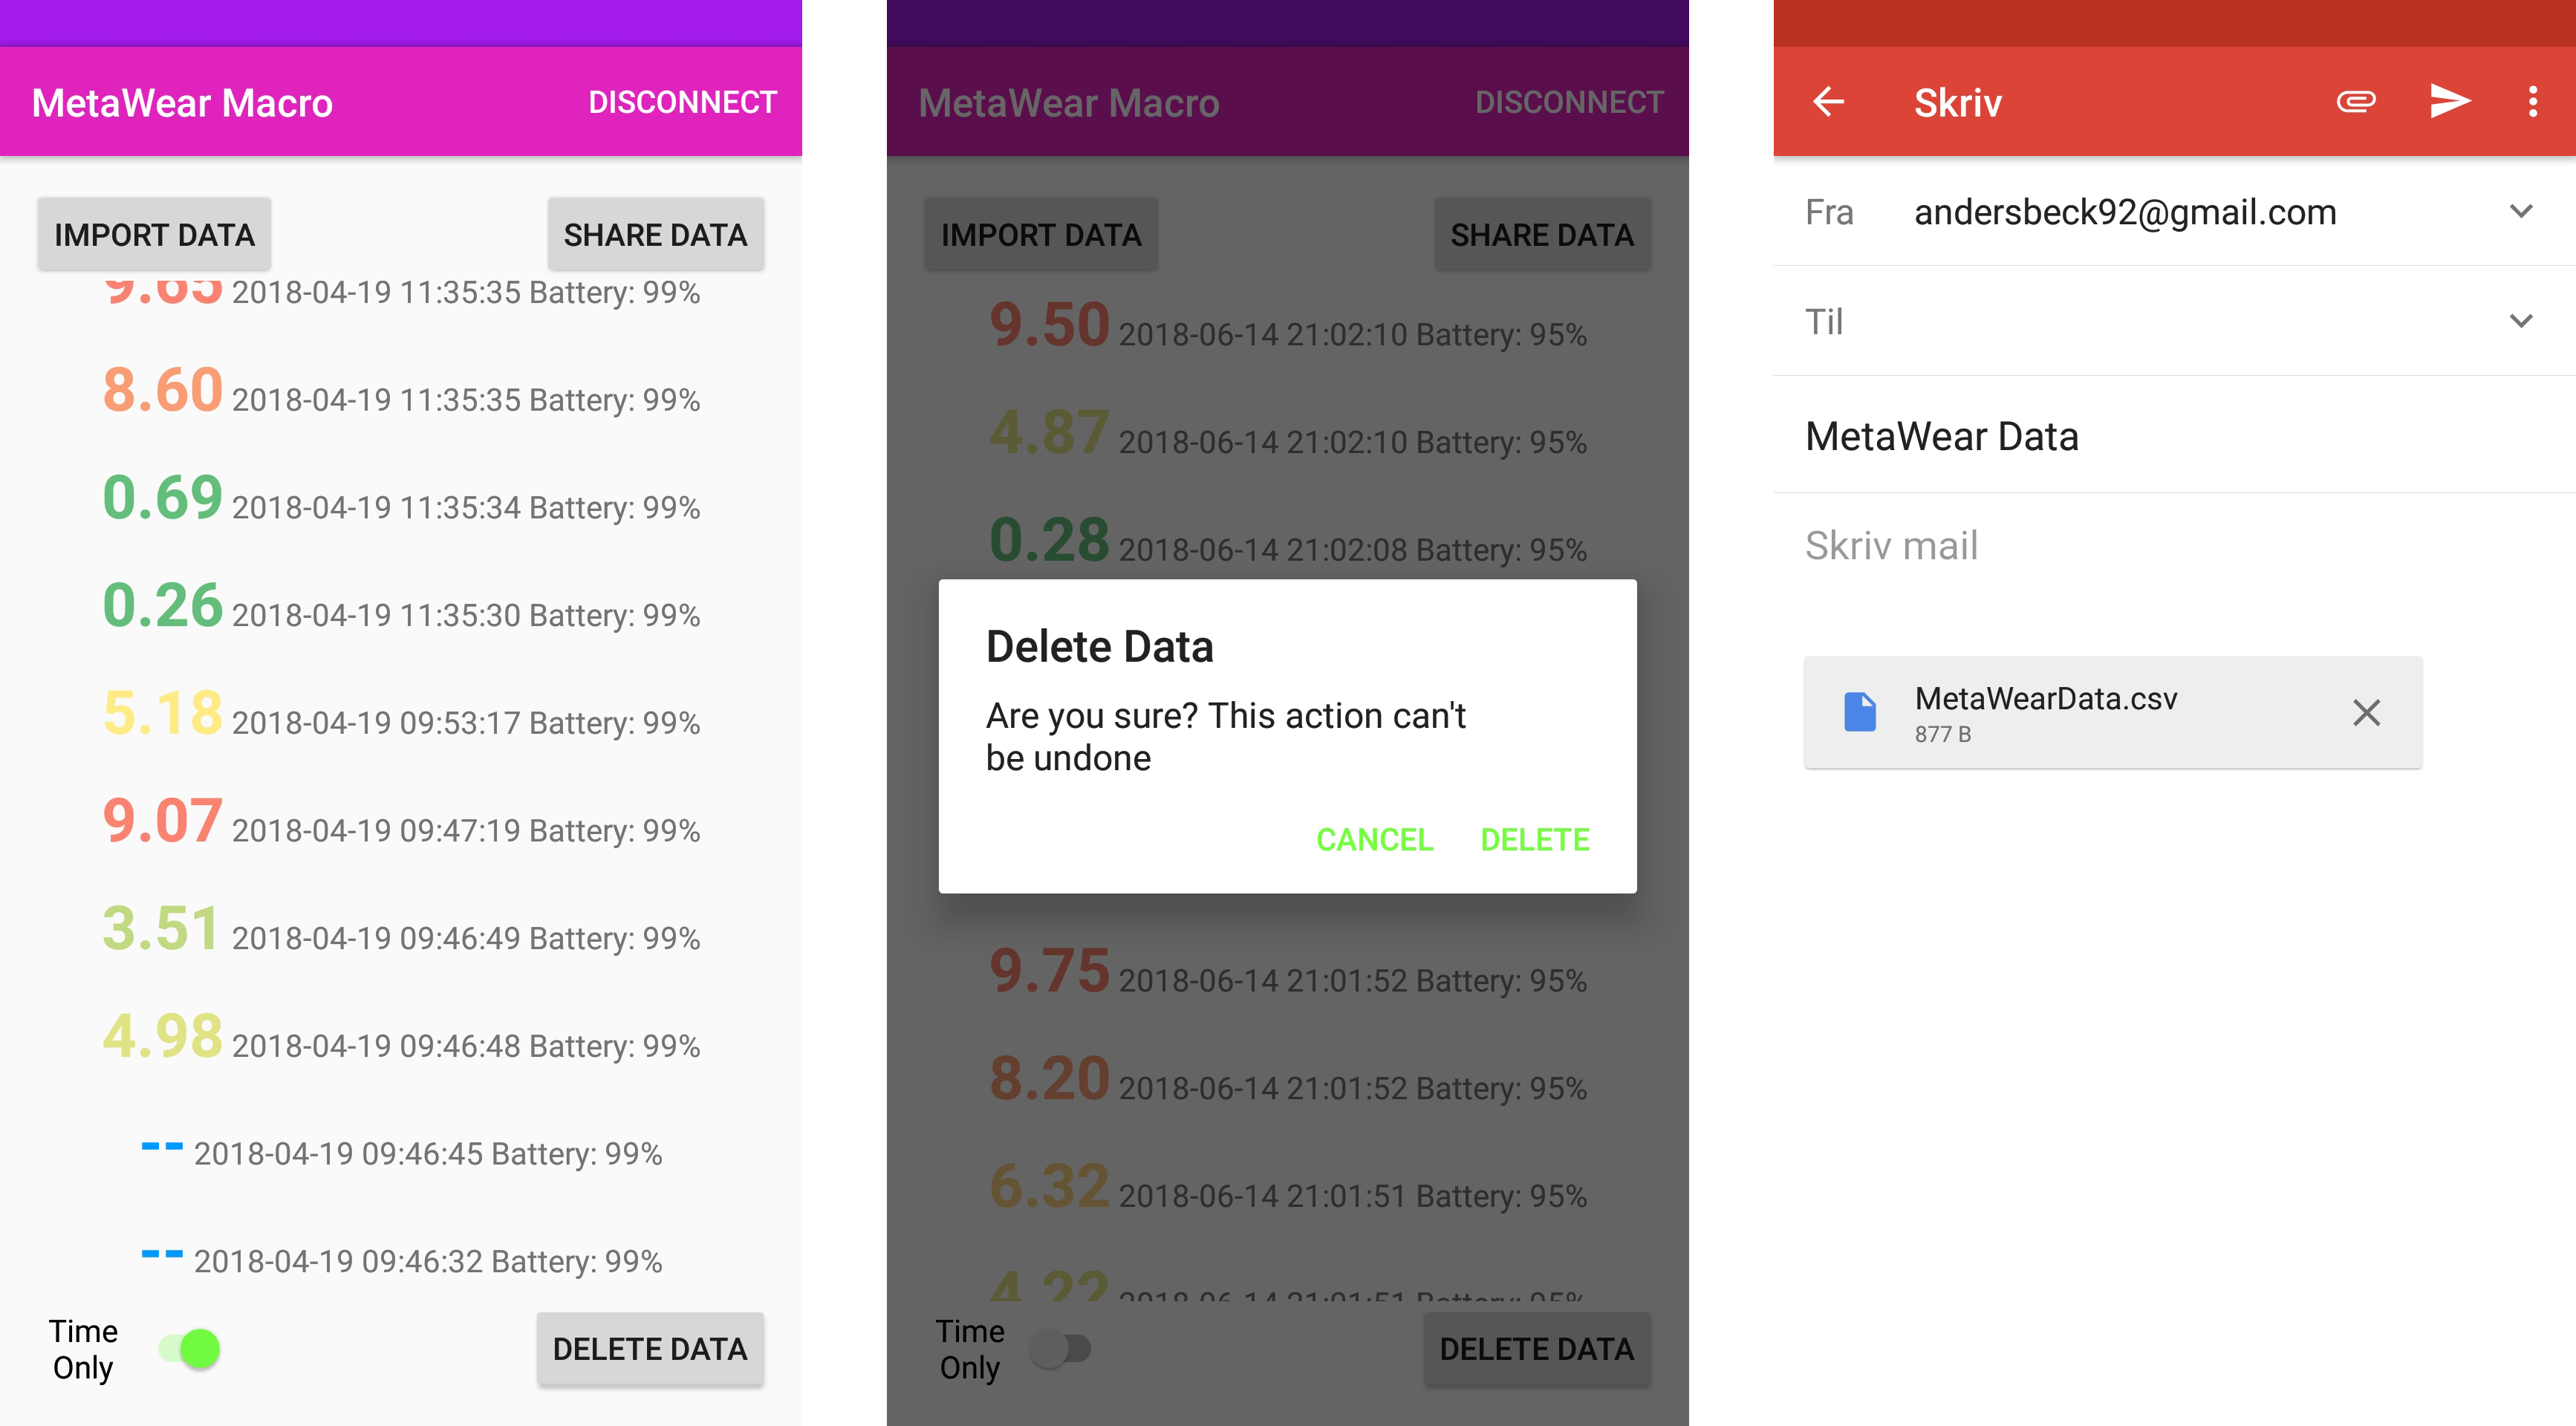
\includegraphics[width=1.1\textwidth]{figures/proto_s1.png}
    \caption{Companion app. Main screen on the left, Delete Data in the middle \& Share Data on the right}
    \label{proto_s1}
\end{figure}



\section{Performance Testing}
The performance of the MetaMotionR and the companion app was tested throughout the implementation process, this was done to ensure that it worked as intended. The first problem that was discovered was related to Sensor Fusion module of the MetaMotionR. Using it the first approach was to only start the algorithm when the button was pressed, measure the Euler angles and then turn the algorithm off waiting for the next button press. The problem turned out to be that the Sensor Fusion algorithm needed a short time to \say{catch up} before it could be used, which resulted in the readings not being accurate, but a little delayed. Solving this problem required the Sensor Fusion algorithm to be turned on at all times, the downside of this is a higher power consumption.

It was then discovered that the battery life of the MetaMotionR was quite limited, depended on the workload. A artificial test was setup to simulate a worst case scenario, the MetaMotionR was programmed to read and transmit the Euler angles to the companion app once every second. The battery percentage was noted at about every 15-30 minutes until the MetaMotionR ran out of battery. The test was run twice, and the results can be seen in Figure \ref{battery_test}, the first test ran for a little less than five hours, while the second time only ran for a little over two hours. These results disappointing, but the test were extreme and real usage would not be that demanding. In order to get a feel of what could be expected by the MetaMotionR in real use, the author choose to wear the device every day for one week, logging entries at least 20 times a day at random times. What was found that with this demand the device could run for at least one day without a charge. It was discovered that the battery percentage would stay in the $\thicksim$90-80\% range through most of the day and night, and once the battery percentage came below $\thicksim$70-60\% it would dramatically drop to zero. Because of this, it was decided to implement the option to disable the logging of orientation, so if this device and app were to be used in real life, one could still get the time stamp recorded which is still valuable information to collect as shown by Larsen et al.\cite{eg}. When used in this mode the battery life is much longer, how long is unknown but it was able to hold a comfortable battery percentage for over a week. One benefit to the battery is that it will fully charge in less than 2 minutes.

\begin{figure}[h!]
    \centering
    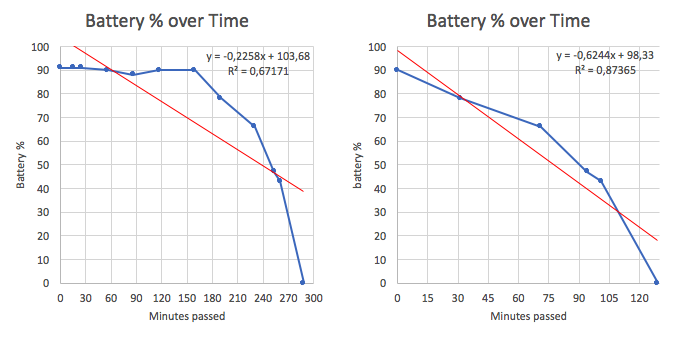
\includegraphics[width=1\textwidth]{figures/batteryTest.png}
    \caption{Battery Tests}
    \label{battery_test}
\end{figure}

